\documentclass[11pt]{article}
\usepackage[margin=1in]{geometry}
\usepackage{fontspec}
\setmainfont{Arial}
\usepackage{graphicx}
\usepackage{booktabs}
\usepackage{multirow}
\usepackage{amsmath}
\usepackage{xcolor}
\usepackage[hidelinks]{hyperref}
\usepackage{caption}
\captionsetup{font=small,labelfont=bf}
\graphicspath{{../figures/}}

% --- Bibliography: biblatex + biber (compiles under XeLaTeX) ---
\usepackage[backend=biber,style=nature,sorting=none,maxbibnames=8,giveninits=true]{biblatex}
\addbibresource{references.bib}

\definecolor{tg}{HTML}{5F6B78}
\newcommand{\msec}[1]{\medskip\noindent{\bfseries\color{tg} #1}\par}

\title{\bfseries A Curated-Ontology Structure-Mapping Memory Turns a Generalist
LLM into a Verifiable Specialist}
\author{Ayaz Khan\\\small Columbia University \quad\texttt{aak2259@columbia.edu}}
\date{2026-06-13 --- working draft for \emph{Nature Machine Intelligence}}

\begin{document}
\maketitle

\begin{abstract}
\noindent Retrieval-augmented generation (RAG) grounds large language models in
external text, but vector and knowledge-graph retrievers index surface similarity
and entity adjacency, discarding the logical structure---subsumption and
higher-order relations---that defines expertise. We present Structure-Mapping
Agentic Memory (SMA), a retrieval memory that encodes each observation as a
functor over a subject and retrieves by analogical structure-mapping against a
curated domain ontology mounted as its ascension lattice. One universal loader
ingests any open OBO/OWL ontology (is-a hierarchy plus
\texttt{someValuesFrom}/\texttt{allValuesFrom} and OBO relationships; no OWL
reasoning)---we mount eleven ontologies spanning seven knowledge areas
($\approx$594{,}000 concepts) and evaluate the memory-swap benchmark on five---with
one shared retrieval core plus thin per-domain data adapters. On a
memory-swap benchmark where only the retriever varies, SMA outperforms a strong
RAG and knowledge-graph baseline suite on the rare, long-tail slice across four
unrelated domains (medicine $+33$, finance $+17$, genomics $+16$, cyber $+7$
percentage points top-5) and on patent classification (legal $+6$, all-query
slice as CPC has no rare split); all five are Holm-significant across domains,
and four of five (medicine, genomics, finance, legal) additionally survive a
conservative selection correction for the data-chosen best baseline, while cyber
is directional ($p_\text{Bonf}=0.17$); SMA matches a
hand-built ontology tool. End-to-end, holding the language model and prompt fixed
and swapping only the memory, the SMA-grounded agent becomes a verifiable
specialist: most accurate, most faithful in citation, and able to separate known
from unknown entities (grounding AUROC $0.79$ versus vector RAG's near-chance
$0.55$), so it abstains and flags novelty. We delimit the thesis honestly: the
advantage is specific to structure and vanishes on flat-tabular prediction.
\end{abstract}

\msec{Main}

Large language models are fluent generalists but unreliable specialists. They
confabulate confidently on the rare, the long-tail, and the high-stakes
cases---precisely where expertise is required and a wrong answer is most
costly~\cite{ji2023hallucination,xiong2024mirage}. The dominant remedy,
retrieval-augmented generation (RAG)~\cite{lewis2020rag}, conditions the model on
documents fetched by embedding similarity~\cite{karpukhin2020dpr} or lexical
overlap~\cite{robertson2009bm25}. This is effective when the answer is frequent
and lexically similar to the query, but it fails on the cases that define
expertise: vector retrieval averages rarity away and indexes surface form, so the
decisive rare term is washed out. Knowledge-graph and graph-RAG
retrievers~\cite{gutierrez2024hipporag,edge2024graphrag} add typed entity edges
but traverse them by path adjacency, still discarding the \emph{subsumption
lattice} (what generalizes to what) and the \emph{higher-order relations}
(relations over relations) that experts actually reason with. The result is a
retriever that cannot tell a known case from an unknown one, and therefore cannot
know when to abstain.

The gap is representational, not a matter of scale. Expertise is organized as
structure: a clinician reasons over an is-a hierarchy of phenotypes and diseases;
an analyst reasons over a typology of techniques and the relations between them.
Decades of cognitive science formalize how humans retrieve and reason over such
structure. Structure-mapping theory~\cite{gentner1983structure} holds that
analogues are aligned by the systematicity of their relational structure rather
than by surface features; the structure-mapping engine (SME) computes consistent
mappings~\cite{falkenhainer1989sme}, and the MAC/FAC model retrieves candidate
analogues tractably from a large memory before aligning
them~\cite{forbus1995macfac,gentner2011computational}. These mechanisms have
never been operationalized as a retrieval memory for grounding language models.

We do so here. SMA treats a curated, open domain ontology as retrieval geometry.
Each observation becomes a functor over a subject; the ontology's is-a tree
becomes an ascension lattice along which specific terms match general ones (with
penalty $\rho^{\mathrm{dist}}$); its typed relations become higher-order
statements; and an information-content scorer ($-\log_2 p$) makes the
rare-but-decisive term dominate by construction. Our thesis is that \emph{a
structure-mapping memory grounded in a curated (expert-maintained) domain ontology turns a generalist
LLM into a verifiable specialist}---beating vector RAG and knowledge graphs on
rare, cross-vocabulary, high-stakes reasoning while supplying provenance,
calibrated abstention, and novelty detection that those retrievers structurally
lack. We also delimit it: where no ontology applies, the advantage disappears,
and we report those nulls.

We make three contributions. First, a \textbf{universal ontology adapter} (loader
+ registry + router), demonstrated on eleven ontologies spanning seven knowledge
areas with one shared retrieval core plus thin per-domain data adapters (gold and
query loaders, no per-domain retrieval logic). Second, a \textbf{memory-swap
benchmark} that holds the language model and prompt fixed and swaps only the
retriever, evaluated against a strong RAG/KG baseline suite. Third, an
\textbf{honest
characterization} of when structure-mapping helps and when it does not.

\begin{figure}[t]\centering
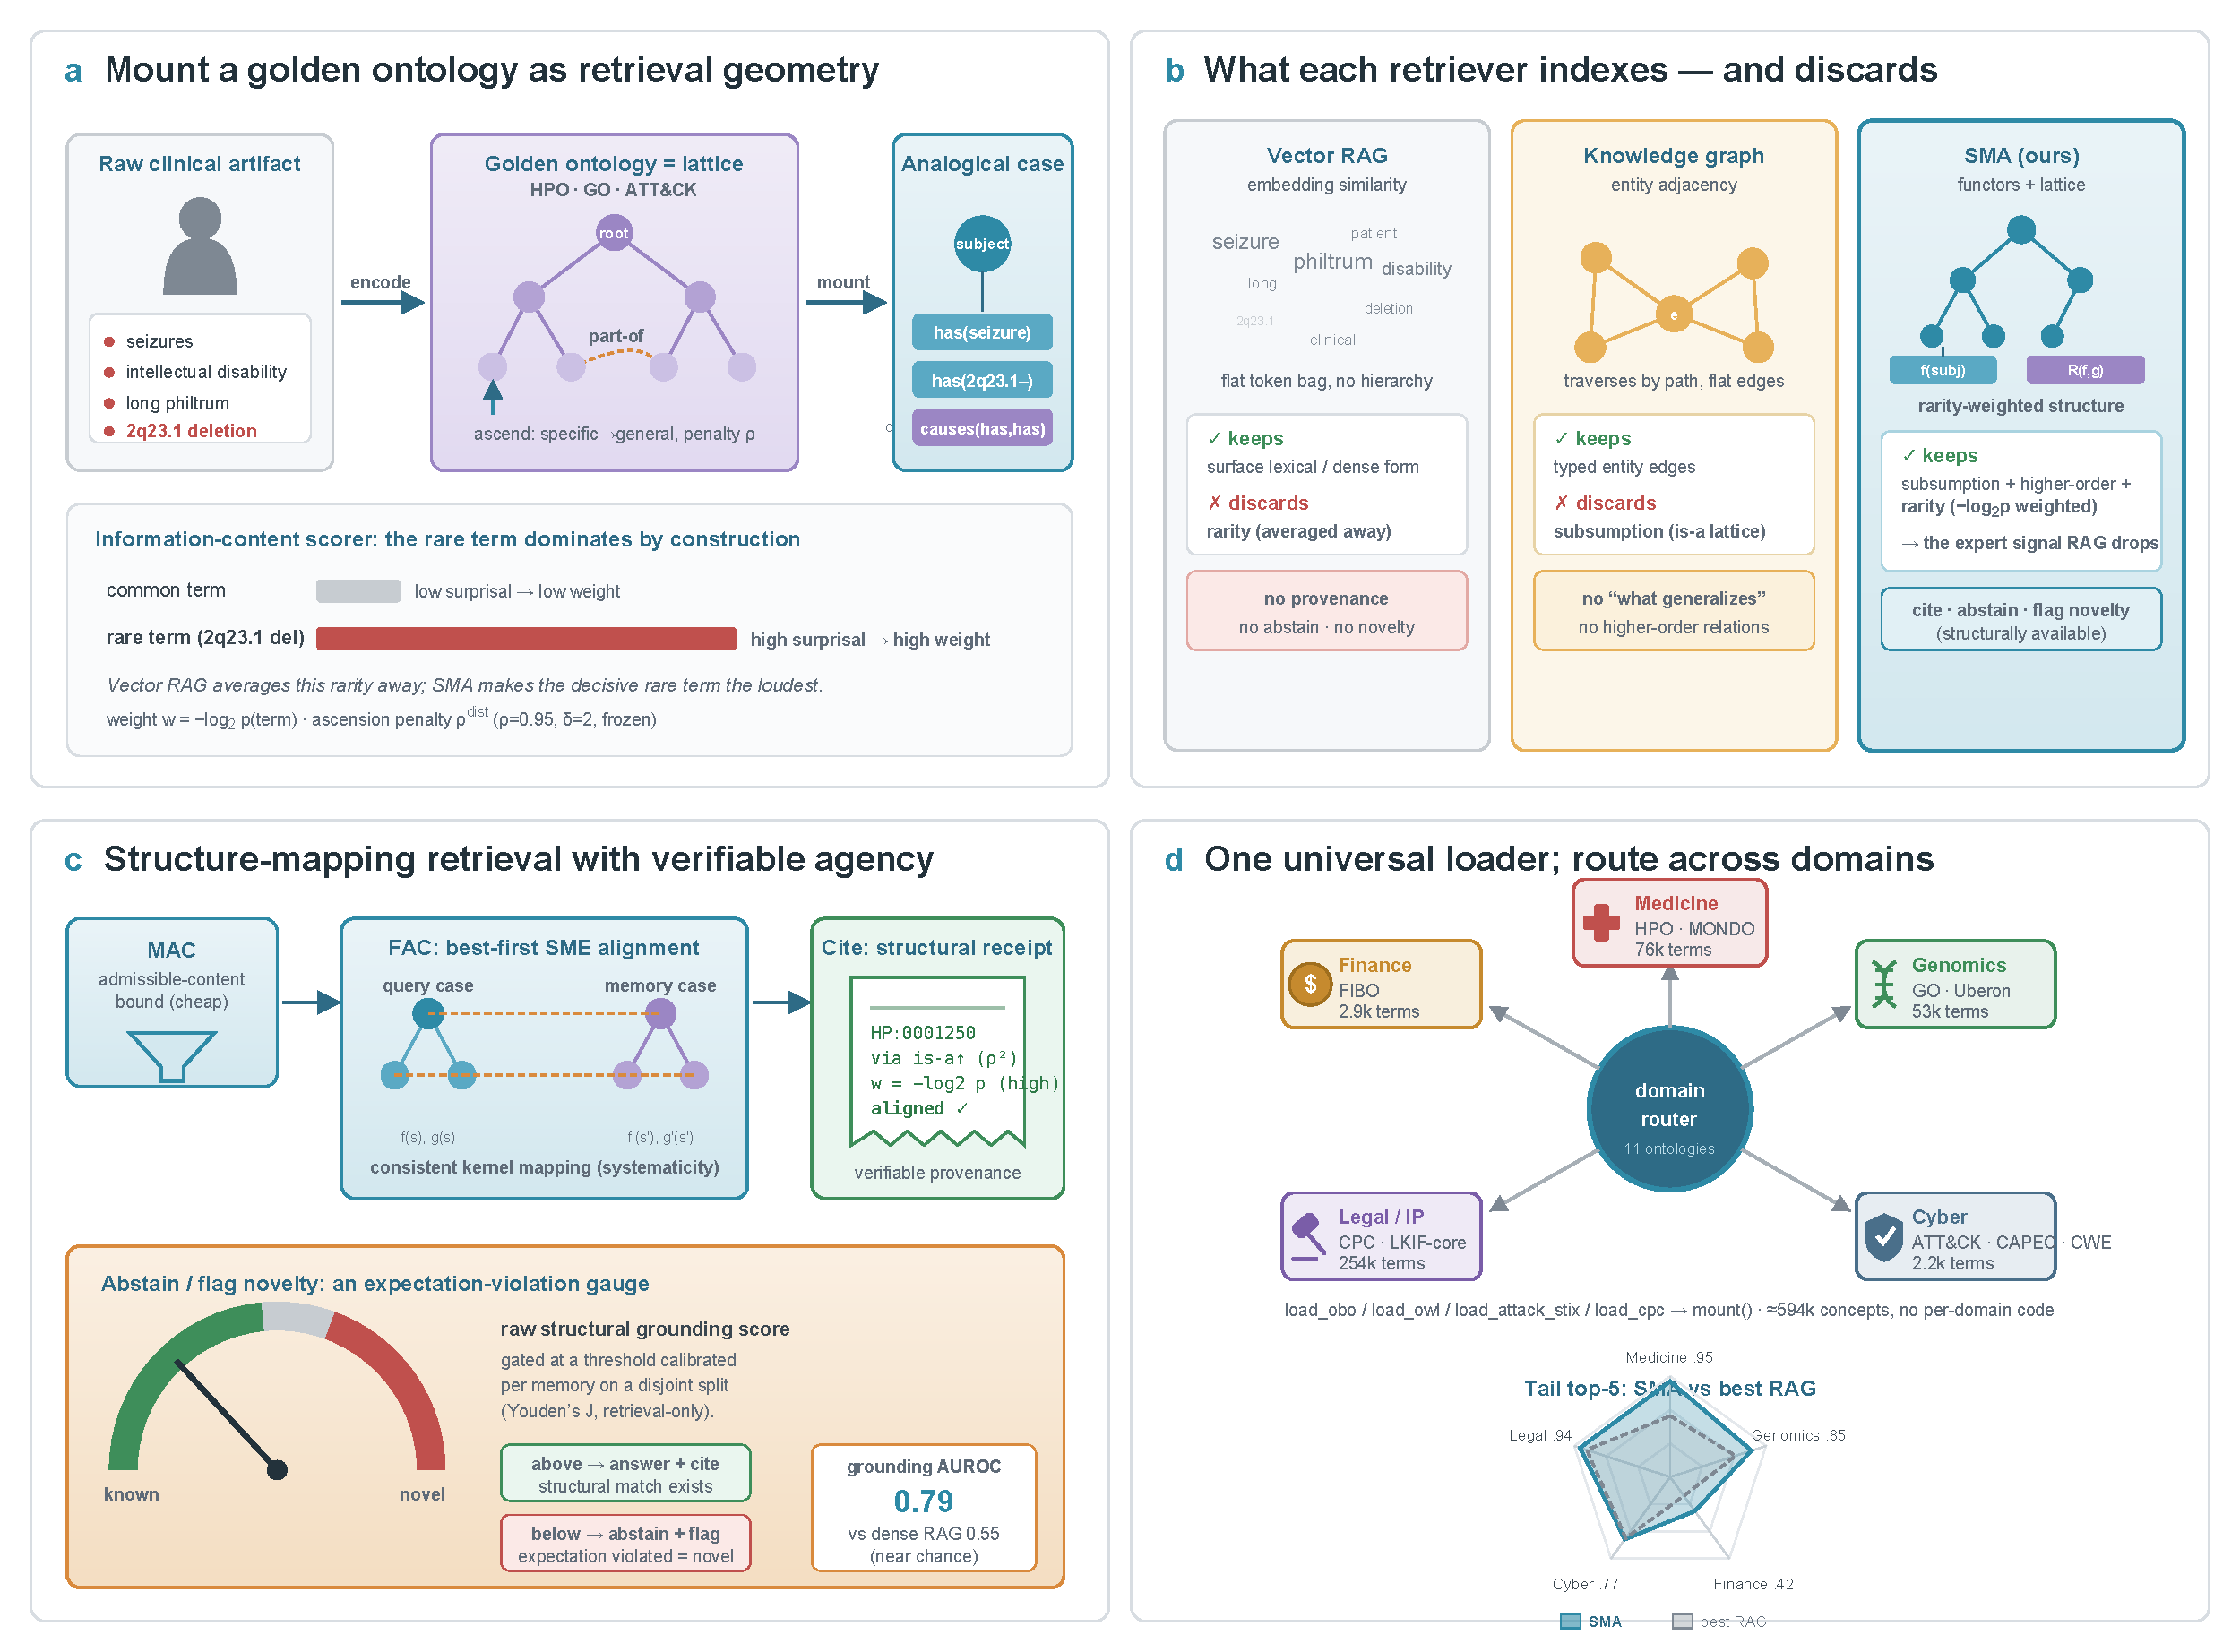
\includegraphics[width=\linewidth]{svg/fig1_overview_v2.pdf}
\caption{\textbf{The universal-adapter system.} (a) Any open ontology is mounted
as retrieval geometry: an artifact is encoded as functors over a subject, the
is-a tree becomes the ascension lattice, and typed relations become higher-order
statements. (b) What each retriever indexes and discards: vector RAG (token
similarity, discards rarity), knowledge graph (entity adjacency, no subsumption),
SMA (functors $+$ lattice, rarity-weighted). (c) Structure-mapping retrieval
(MAC bound $\to$ FAC alignment) with structural citation and abstention: a
structural citation and an abstain/novelty signal from expectation violation.
(d) One universal loader mounts eleven ontologies spanning seven knowledge areas;
a domain router routes across the evaluated domains without merging them.}
\end{figure}

\msec{Results}

\textit{The universal adapter and the memory-swap protocol.} The loader parses
any OBO/OWL/STIX/CPC source into a normalized ontology graph, mounts the is-a
tree as the ascension lattice and the typed relations as higher-order statements,
and indexes each entity's term-set as an analogical case (Table~1). A registry
and a domain router select the relevant ontology per query, so a single mechanism
serves all five evaluated domains without merging them. The benchmark holds the
language model and prompt fixed and swaps only the retrieval memory among SMA and
the baseline retrievers, so any difference is attributable to retrieval alone. The
baseline retrieval suite is: BM25~\cite{robertson2009bm25}, BGE neural dense
retrieval~\cite{karpukhin2020dpr}, hybrid reciprocal-rank fusion, hybrid with a
cross-encoder reranker, and the graph retriever
HippoRAG~\cite{gutierrez2024hipporag}. We score the rare/long-tail slice
(entities whose rarest term has information content above the corpus median),
where expertise is decisive, with a paired bootstrap ($10^4$ resamples) and
Holm--Bonferroni correction across domains.

\textit{SMA matches a bespoke ontology oracle but outperforms general-purpose RAG/KG.}
A retriever that consumes the same ontology should be near-optimal on
pure-subsumption ranking, and one is: against Phenomizer~\cite{kohler2009phenomizer},
a hand-built ontology-aware information-content tool that scores the same
Resnik~\cite{resnik1995} information content SMA uses, SMA reaches statistical
parity on top-5 (HPO $\Delta{=}{-}0.033$, $p{=}0.037$, Holm $p{=}0.073$;
GO $\Delta{=}{-}0.011$, $p{=}0.71$): SMA matches but does not beat the bespoke
oracle. This parity is the direct rebuttal to ``SMA merely optimises information
content'': Phenomizer is an IC-similarity oracle built on the identical
$\mathrm{IC}=-\log_2(c/n)$ weighting, yet SMA only ties it while decisively
outperforming the IC-agnostic BM25/dense/hybrid suite (Fig.~2, Table~2). IC
weighting is therefore necessary but not what separates SMA from RAG; the
ascension lattice and higher-order structural alignment are. We frame the oracle
as a ceiling reference, not an opponent, and state the headline claim as
\textbf{SMA $>$ RAG/KG}.

\textit{A structure-only control isolates the mechanism from lexical and information-content
similarity.} One concern is that SMA's advantage merely reflects information-content weighting
or lexical overlap that a tuned retriever could recover. We rebut this directly with the
Synthetic Structure Benchmark (SSB), an adversarial control in which structure is the
\emph{only} usable signal. Each query and its correct library entry are zero-lexical-overlap
relational analogs bridged solely through the ascension lattice: they share no surface tokens,
so BM25 and TF-IDF/dense retrieval are information-theoretically blind, and the gold match is
recoverable only by aligning higher-order relational structure across the lattice. On the
$200$ pooled library queries ($100$ queries $\times\,2$ seeds), SMA attains rank-1 accuracy
$0.895$ (MRR $0.948$), whereas both BM25 and TF-IDF/dense retrieval score $0.000$ at rank-1
(MRR $\approx 0.010$, at chance): $\Delta\,r@1{=}{+}0.895$, 95\% CI $[0.850, 0.935]$,
$p_{\mathrm{Holm}}{=}4{\times}10^{-4}$, Cliff's $\delta{=}0.895$ against each lexical/dense
baseline. In the forced-choice variant, where each query is paired against a single structural
distractor, SMA reaches rank-1 $1.000$. The control is de-circularized---the earlier
\texttt{far\_}-prefix bijection and $(i, i{+}2)$ rewiring were removed, so no shortcut maps
queries to entries by surface convention. Because SSB carries no information-content gradient
for either retriever to exploit and is lexically orthogonal by construction, the result
separates SMA's structure-mapping mechanism from both lexical overlap and information-content
similarity: the win is structural, not lexical, and not an artifact of information-content
weighting alone (Extended Data Table~3).

\textit{The edge is structure-mapping, not ancestor expansion.} A natural
objection is that SMA wins merely because it sees each term's is-a ancestors,
which the baseline retrievers do not. We tested this directly by giving BM25 and
dense retrieval the same advantage: every document and query term-set was
expanded with its full is-a ancestor closure before indexing
(rare-slice top-5; Extended Data Table~4). Ancestor expansion \emph{hurts} the
retrievers rather than helping them---on GO, BM25 falls from $0.776$ to $0.504$
and dense from $0.719$ to $0.465$; on HPO the same arms move from $0.731$ to
$0.715$ and from $0.622$ to $0.561$---because the shared common ancestors are
high-frequency, low-information terms that dilute the IDF and cosine signal that
the rare, decisive term would otherwise carry. SMA still beats every
ancestor-expanded arm by Holm-significant margins (HPO $+0.20$ versus
BM25$+$ancestors and $+0.36$ versus dense$+$ancestors; GO $+0.34$ and $+0.38$;
all $p_{\mathrm{Holm}}{=}0.0012$). The one honest nuance is on GO, where
\emph{unexpanded} BM25 reaches parity with SMA ($\Delta{=}{+}0.070$,
$p_{\mathrm{Holm}}{=}0.076$, n.s.); on HPO and on every expanded arm SMA's lead
is significant. Structure-mapping over the ascension lattice, not raw ancestor
expansion of the retrievable text, is therefore what produces the advantage.

\textit{Across the baseline retrieval suite, SMA wins on the tail across fields}
(Fig.~2, Table~2). On \textbf{medicine} (rare-disease diagnosis over the Human
Phenotype Ontology~\cite{kohler2021hpo} and MONDO~\cite{vasilevsky2022mondo}) SMA
attains tail top-5 of $0.949$ versus $0.606$ for the best baseline
configuration (hybrid $+$ cross-encoder rerank), $\Delta{=}{+}0.333$, 95\% CI
$[0.281,0.389]$, $p{<}2{\times}10^{-4}$. On \textbf{genomics} (Gene
Ontology~\cite{ashburner2000go,geneontology2021} gene-function assignment) SMA
reaches $0.849$ versus $0.682$, $\Delta{=}{+}0.156$, $p{<}2{\times}10^{-4}$. On
\textbf{finance} (SEC filing to US-GAAP concept) SMA attains $0.418$ versus
$0.231$, $\Delta{=}{+}0.167$, $p{<}2{\times}10^{-4}$---roughly double the best
RAG, though all methods score low here because US-GAAP concepts are weakly
discriminative. On \textbf{legal} (patent to CPC classification, all-query slice)
SMA reaches $0.941$ versus $0.870$, $\Delta{=}{+}0.064$, $p{=}0.002$. On
\textbf{cyber} (MITRE ATT\&CK~\cite{strom2018attack} threat-group attribution)
SMA leads $0.766$ versus $0.749$, $\Delta{=}{+}0.073$, $p{=}0.035$---a smaller
margin, honestly attributable to threat groups' distinctive technique
vocabularies, which lexical and dense retrieval partly capture. All \textbf{five}
unrelated domains survive Holm correction across fields,
confirming the pre-registered across-fields criterion. Because ``best RAG'' is
data-selected (chosen by top-5 then tested on top-5), we additionally compare
SMA against \emph{every} baseline in \emph{every} domain: the advantage is
strictly positive in all cases, and under a conservative
Bonferroni-over-baselines correction four of five domains survive (medicine,
genomics, finance at $p_\text{Bonf}{=}0.0010$, legal at $0.0110$) while cyber is
directional ($p{=}0.035$, $p_\text{Bonf}{=}0.17$; Extended Data Table~8). (Legal's rare slice is undefined: CPC's near-uniform
information content yields no rare split, so legal is reported on the all-query
slice and flagged as such.)

\begin{figure}[t]\centering
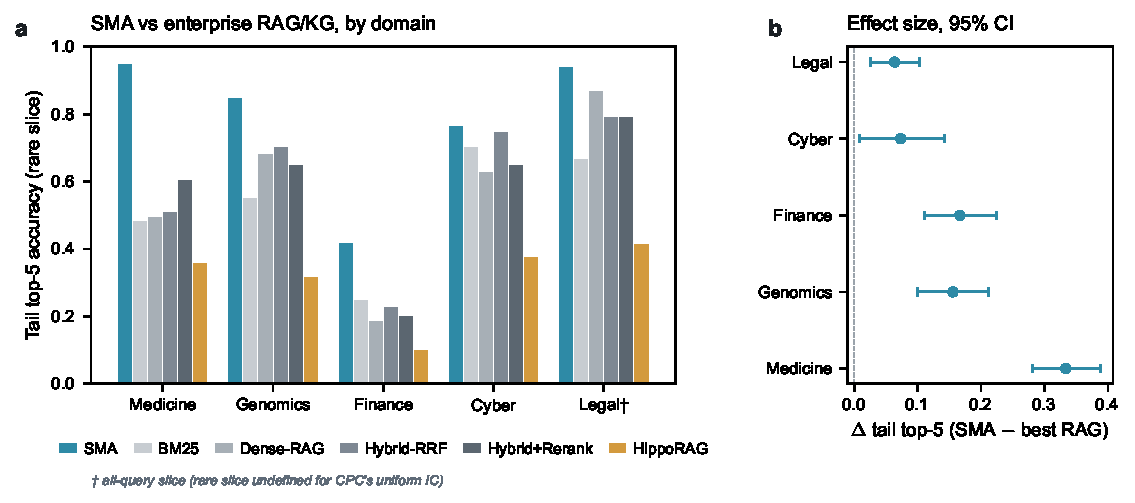
\includegraphics[width=\linewidth]{svg/figure2_results.pdf}
\caption{\textbf{Agentic memory-swap results.} (a) Tail top-5 accuracy (rare
slice; legal on the all-query slice) by domain: SMA versus the RAG/KG baseline
suite. (b) Headline effect size $\Delta$(SMA $-$ best RAG) tail top-5 per domain
with 95\% CI; all above zero. AURC and structural-novelty F1 per domain are in
Table~2(b) and Extended Data Fig.~1.}
\end{figure}

\textit{Cite-or-abstain and structural novelty.} SMA has the lowest
risk-coverage area-under-the-risk-coverage-curve (AURC) in every one of the five
arms ($0.017$--$0.530$ versus best-RAG $0.261$--$0.857$): a structural match
either exists or it does not, whereas cosine similarity is always moderately
high, so a pure-RAG retriever cannot tell when to abstain. On held-out unknown
entities SMA's expectation-violation flag yields a structural-novelty F1 of
$\approx 0.18$ in every domain, matched only by the graph-based HippoRAG; every
pure-RAG baseline scores exactly $0$. Absolute novelty F1 is reported honestly:
the retrieval-suite threshold is fixed and untuned, so the contrast that matters
is non-zero versus structurally zero, not the absolute level (the end-to-end
agent below calibrates the threshold per memory).

\textit{The end-to-end agent is a verifiable specialist.} The retrieval suite
isolates the retriever; we next place a real language model in the loop and
measure what matters in deployment, where a confident wrong answer is
catastrophic. Holding the language model (DeepSeek, temperature $0$) and the
prompt fixed and swapping only the memory (closed-book / dense-RAG / SMA), an
ontology-grounded diagnosis agent answered $120$ \emph{answerable}
(indexed-disease) and $120$ \emph{held-out} (unseen-disease) clinical cases, with
a cite-or-abstain threshold calibrated per memory on a \emph{disjoint} split
(pre-registration~v2; Methods). The SMA-grounded agent dominates the
trustworthy-QA composite (Fig.~3). It is the most accurate ($0.342$ versus dense
$0.100$ versus closed-book $0.017$; paired-bootstrap $\Delta{=}{+}0.242$, 95\% CI
$[0.167,0.325]$, Holm-significant) and the most faithful in citation (ALCE-style
support~\cite{gao2023alce} $0.621$ versus $0.480$). Decisively, its raw
structural grounding score separates known from unknown entities (AUROC $0.793$
versus dense's near-chance $0.547$; $\Delta{=}{+}0.246$, $[0.159,0.333]$): cosine
similarity stays high even for unseen diseases, so dense RAG can reach
abstain-recall $0.90$ only by refusing $79\%$ of answerable cases, whereas SMA
reaches $0.91$ while refusing $45\%$. Abstain-recall itself is therefore a
\emph{tie} ($\Delta{=}{+}0.008$, $p{=}0.92$); we report it as such. The net
selective accuracy is $0.625$ versus $0.500$ ($\Delta{=}{+}0.125$,
$[0.071,0.179]$) and structural-novelty F1 is $0.789$ versus $0.553$
(novelty-recall $\Delta{=}{+}0.308$, $[0.200,0.408]$); closed-book scores $0$ on
novelty and cannot cite at all. Four of five pre-registered axes are
Holm-significant wins, abstain-recall is a tie, and the accuracy floor holds (SMA
above, not below, RAG). Equipped with structure-mapping memory, a generalist LLM
answers, cites, abstains, and flags novelty; equipped with vector RAG, it answers
less accurately and cannot tell when it does not know.

\begin{figure}[t]\centering
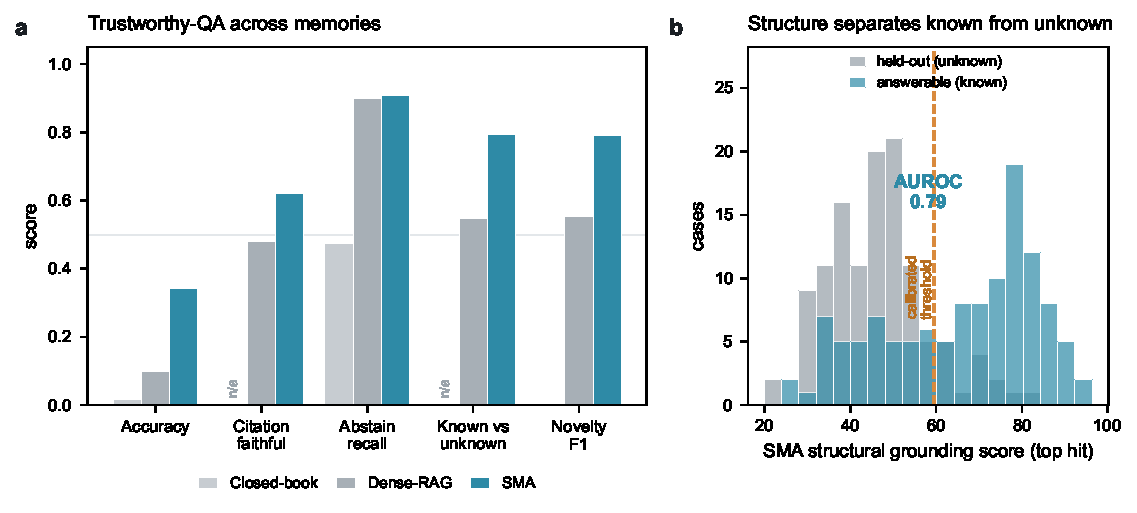
\includegraphics[width=\linewidth]{svg/figure5_trustworthy.pdf}
\caption{\textbf{The SMA-grounded LLM agent is a verifiable specialist}
(medicine; $n{=}120$ answerable ${+}\,120$ held-out; language model and prompt
fixed, memory swapped). (a) Trustworthy-QA axes for closed-book / dense-RAG /
SMA: accuracy, citation-faithfulness, abstain-recall, known-versus-unknown
discrimination (grounding AUROC), and novelty F1; closed-book has no retrieval,
so its citation and grounding cells are N/A (marked), not zero. (b) Mechanism:
SMA's raw structural grounding score (top hit) separates answerable (known) from
held-out (unknown) cases, AUROC $0.79$; the dashed line is the cite-or-abstain
threshold calibrated on a disjoint split. Dense cosine similarity barely
separates the two (AUROC $0.55$), forcing its gate to over-abstain.}
\end{figure}

\textit{Negative results and boundary.} We pre-registered a parity-reporting
rule: where a task carries no discriminative subsumption ontology to mount, we
report parity or a null rather than search for an edge. Two families satisfy this
condition. First, \textbf{flat single-record tabular prediction}: on hospital
readmission and credit-card fraud, each record is encoded independently and the
discriminative structure is cross-record, so SMA reaches parity with value-based
retrieval and goes no further. We verified the mechanism directly---an
LLM-drafted higher-order adapter mechanically raised relation density from $0$,
yet lifted SMA only to parity with dense retrieval, not past it. Second, as a
follow-up boundary probe, we asked whether \emph{graph} structure alone suffices
when single-record structure does not. On the public Elliptic Bitcoin
ledger~\cite{weber2019elliptic} we encoded each transaction's graph
neighbourhood---predecessor and successor flows---as higher-order relations over
a licit/illicit typology lattice, with strict label-leak guards, supplying the
cross-record structure that flat-tabular retrieval lacks and that graph neural
networks~\cite{kipf2017gcn} exploit. The outcome is an honest null: SMA shows no
significant edge over dense or lexical retrieval ($\Delta$ accuracy $+0.004$,
95\% CI $[-0.010,+0.019]$, $p{=}0.56$), and \emph{every} retrieval method---SMA
included---trails a flat logistic-regression baseline on the full $166$-feature
record (macro-F1 $0.787$ versus SMA's $0.581$; Extended Data
Table~5). The lesson sharpens the thesis: graph topology
alone is not enough. A coarse licit/illicit typology yields too few distinct
structural signatures for analogical alignment to beat vector similarity;
structure helps SMA only when the subsumption ontology is itself richly
differentiated, as in the curated (expert-maintained) ontologies. We draw the
boundary rather than hide it: SMA needs a discriminative subsumption ontology,
not mere graph topology.

\msec{Discussion}

One mechanism serves medicine, genomics, finance, legal and cyber with one shared
retrieval core plus thin per-domain data adapters (no per-domain retrieval
logic)---a generality the bespoke ontology tools (one per domain) cannot match.
The defensible asset is a registry of curated (expert-maintained) ontologies
mounted as retrieval geometry; a language model can draft adapter rules but does
not reproduce the expert curation encoded in the ontology. Relational richness,
not raw size, appears to drive SMA's edge over the information-content oracle:
pure-is-a ontologies (HPO, CPC) yield parity, whereas relation-rich ones should
let higher-order structure-mapping pull ahead---an open, testable prediction.

Limitations. The retrieval-suite novelty threshold is fixed and untuned (the
end-to-end agent calibrates it per memory on a disjoint split). HippoRAG is
somewhat disadvantaged by a bag-of-term-names document representation that suits
its phrase-graph poorly. The interactive end-to-end study is a single-domain
(medicine) case study. We restrict to fully open ontologies and exclude licensed
sources (SNOMED, UMLS) in favour of reproducibility.

\textit{What we do not claim.} We state the boundaries of the thesis
explicitly. \textbf{(i)}~We claim no advantage on flat, single-record
tabular prediction: hospital readmission and credit-card fraud reach only
parity with value-based retrieval, and on the Elliptic Bitcoin
ledger~\cite{weber2019elliptic} SMA shows no significant edge over the best
retrieval baseline ($\Delta$ accuracy $+0.004$, 95\% CI $[-0.010,+0.019]$,
$p{=}0.56$), with all retrieval methods trailing a flat logistic-regression
baseline---there is no ontology structure to exploit.
\textbf{(ii)}~We do not claim to beat the bespoke ontology oracle
Phenomizer~\cite{kohler2009phenomizer}: on pure-subsumption ranking SMA
reaches parity only (HPO $\Delta{=}{-}0.033$, GO $\Delta{=}{-}0.011$; Holm
n.s.), matching but not exceeding a hand-built information-content tool. The
headline win is over ontology-agnostic RAG/KG, not over the oracle.
\textbf{(iii)}~The end-to-end LLM-in-the-loop study is medicine-only; the
broader memory-swap results are retrieval-only.
\textbf{(iv)}~The retrieval-suite structural-novelty threshold is fixed and
untuned, so its absolute novelty F1 is not a tuned operating point (only the
end-to-end agent calibrates the threshold per memory).
\textbf{(v)}~We restrict to fully open ontologies and exclude licensed
vocabularies (SNOMED, UMLS) in favour of reproducibility, so we make no claim
about coverage those sources would add.
\textbf{(vi)}~This is a \emph{representational} claim---structure as retrieval
geometry---not a claim about model scale or fine-tuning; the language model and
prompt are held fixed throughout and only the memory is swapped.
\textbf{(vii)}~In our mechanism ablation, higher-order typed relations did not
add measurable tail top-5 accuracy beyond is-a subsumption combined with
information content; the gain we report is attributable to subsumption and
IC weighting, not to relations over relations.

\textit{Relation to prior work.} Grounding LLM memory in ontologies is an active
2024--2026 area; our contribution is not ontology-grounding per se but the
structure-mapping mechanism and the universal adapter that mounts any curated
ontology as match geometry. Information-content semantic-similarity measures
(Resnik~\cite{resnik1995}; Lin~\cite{lin1998}; Jiang--Conrath~\cite{jiang1997})
score term-set overlap weighted by corpus frequency; SMA instead aligns
relational statements $r(f_s(x),f_o(x))$ over the ascension lattice. Tellingly,
the IC oracle Phenomizer~\cite{kohler2009phenomizer} uses this same information
content, yet SMA only \emph{matches} it (HPO $\Delta{=}{-}0.033$,
GO $\Delta{=}{-}0.011$; parity after Holm) while still beating the IC-agnostic
retrieval suite---so IC weighting is not what produces SMA's advantage. Ontology-
and knowledge-graph-aware retrieval---OG-RAG~\cite{ograg2024} and
OntologyRAG~\cite{ontologyrag2025}, and the KG-RAG line of
GraphRAG~\cite{edge2024graphrag} and HippoRAG-2~\cite{gutierrez2025hipporag2}---%
flatten the ontology into retrievable text or an OpenIE-derived phrase graph;
SMA instead mounts the asserted lattice directly as typed match geometry, with no
OpenIE step and no per-domain retrieval code. Finally, unlike case-based
reasoning over LLM memories (CBR-RAG~\cite{cbrrag2024}), where retrieval reduces
to surface feature similarity, SMA's first stage is structural alignment under an
admissible MAC bound~\cite{forbus1995macfac}. Specialised biomedical tooling
(the Ontology Access Kit~\cite{oak}; Exomiser~\cite{exomiser}) realises
ontology-aware similarity within single domains; SMA supplies one shared
mechanism across all of them.

\msec{Methods}

\textit{Representation and matching.} Statements are functors over entities; SME
builds consistent kernel mappings~\cite{falkenhainer1989sme}; MAC/FAC provides a
certified admissible content bound for tractable first-stage retrieval and
best-first alignment for the second~\cite{forbus1995macfac}. Cross-vocabulary
matching ascends the ontology lattice with penalty $\rho^{\mathrm{dist}}$ (frozen
$\rho{=}0.95$, ascension depth $\delta{=}2$). The surprisal scorer weights a
matched functor by its information content $-\log_2 p$.

\textit{Cases as functored statements.} The loader encodes each subject (an
entity record) as a \emph{case}: a set of logical statements. Each present
ontology term $T$ on a subject $x$ is the unary statement $f_T(x)$, and each
asserted typed relation $(s,r,o)$ whose endpoints $s$ and $o$ are both present
on $x$ becomes the higher-order statement $r\!\left(f_s(x),f_o(x)\right)$---a
relation over relations. A case is the set of all such statements for $x$. Here
``functor'' denotes a predicate / term-constructor symbol in the
structure-mapping sense---it labels a statement and may take statements as
arguments---and is \emph{not} a category-theory functor; this higher-order
constructor is what lets SME align relations between
relations~\cite{falkenhainer1989sme}. Subsumption is not materialized at load
time: the loader extracts the asserted is-a DAG plus the typed relations into a
single normalized graph, and generalization is realized only at match time by
bounded $\delta$-hop ascension over asserted edges (no OWL reasoner is invoked).
Multi-parent DAGs are supported, cyclic is-a chains are truncated at depth
$\delta$, and OWL axioms beyond \texttt{subClassOf} and existential / universal
(\texttt{someValuesFrom} / \texttt{allValuesFrom}) restrictions are not consumed.

\textit{Ascension and information content.} A specific term matches a more
general one along the lattice with factor
\begin{equation}
a(m)=\rho^{\,\mathrm{dist}(m)},\qquad \mathrm{dist}(m)\le\delta,
\end{equation}
where $\mathrm{dist}(m)$ is the minimal is-a distance between the matched terms
and a match beyond $\delta$ hops is disallowed (frozen $\rho{=}0.95$,
$\delta{=}2$). Information content is the Resnik information-content
estimate~\cite{resnik1995} from corpus term
frequency with is-a closure propagation,
\begin{equation}
\mathrm{IC}(c)=-\log_2\!\frac{\mathrm{count}(c)}{n},
\end{equation}
where $\mathrm{count}(c)$ accumulates every annotation of $c$ and of its is-a
descendants and $n$ is the corpus total; the surprisal scorer sets a matched
functor's base weight to its surprisal $\sigma_0(m)=-\log_2 p(m)$ (and to $1$
when the functor is uncosted), so the rare-but-decisive term dominates by
construction.

\textit{Trickle-down structural score.} The structural support of a case is the
sum over match hypotheses $m$ of a trickle-down score in which a hypothesis
inherits a discounted share of the support of the hypotheses it is an argument
of,
\begin{equation}
S(m)=\sigma_0(m)\,a(m)+\gamma\!\!\sum_{p\in\mathrm{parents}(m)}\!\!S(p),
\end{equation}
with discount $\gamma{=}0.25$; $\mathrm{parents}(m)$ are the hypotheses whose
aligned arguments are $m$, so systematic (deeply nested) structure compounds
while isolated term matches do not. Setting the functor costs to none recovers a
uniform-weight structural evaluation ($\sigma_0\equiv1$).

\textit{Admissible content bound.} First-stage MAC retrieval ranks candidates by
an admissible upper bound on the structural score that never underestimates the
true alignment, so no true match is pruned:
\begin{equation}
U(q,c)=\bar s\sum_{f}\mathrm{cost}(f)\,\min\!\bigl(q_f,c_f\bigr),
\end{equation}
where $q_f$ and $c_f$ are the functor-$f$ counts of the query and candidate
content vectors and $\bar s{=}4.0$ is the per-match-hypothesis score ceiling in
production. Only the bounded shortlist is passed to the FAC alignment
stage~\cite{forbus1995macfac}.

\textit{Novelty by expectation violation.} A held-out case is flagged as novel by
its expectation violation against the indexed schemas,
\begin{equation}
\mathrm{ev}(\mathrm{case})=1-\max_{g}\;\mathrm{fit}_{\mathrm{norm}}\!\bigl(\mathrm{case},\mathrm{schema}_g\bigr),
\end{equation}
where $\mathrm{fit}_{\mathrm{norm}}\in[0,1]$ is the normalized structural-match
score of the case against learned generalization $g$; $\mathrm{ev}=1$ when no
generalization yet exists (nothing is expected). Novelty is thus detected from
structural mismatch, not from term absence.

\textit{Citation faithfulness.} Citation faithfulness is computed automatically as
an exact structural identifier match: among answerable items that the agent
answered (did not abstain on) and cited, the fraction whose cited candidate
identifier equals the gold identifier. It is therefore an ALCE-style
support~\cite{gao2023alce} \emph{proxy} based on structural attribution, not an
entailment / NLI judgement. Because it conditions on answered items only, it is
reported alongside but not on the same denominator as accuracy (e.g.\ $0.621$
faithfulness over cited answers versus $0.342$ accuracy over all answerable
cases).

\textit{Language-model decoding and failure semantics.} The end-to-end agent
queries DeepSeek (\texttt{deepseek-chat}) with temperature $0$,
\texttt{max\_tokens}${=}600$, a single attempt, a $60$\,s timeout and no retries;
the temperature-$0.3$ verbalizer path is not exercised by the QA harness. Each
reply is parsed as strict one-line JSON, and any parse, type or range failure
collapses deterministically to \textsc{abstain}, the safe action, so a
malformed completion is never scored as an answer.

\textit{Universal adapter.} The loader (\texttt{sma/ontology}) provides
\texttt{load\_obo/load\_owl/load\_owl\_dir/load\_rdflib/load\_attack\_stix/}
\texttt{load\_cpc/load\_mitre\_xml}; \texttt{mount()} builds the lattice and the
case builder; a registry and a domain router select the ontology per query.
Ontologies are version-pinned, and \texttt{PYTHONHASHSEED=0} with sorted
set$\to$list conversion ensures process-independent reproducibility.

\textit{Memory-swap retrieval benchmark.} The harness (\texttt{sma/eval/agentic})
wraps SMA and each baseline behind one interface, indexes identical records,
generates hard partial/imprecise/noisy queries, and scores tail top-$k$ (rare
slice $=$ rarest-term information content above the corpus median), risk-coverage
AURC, and structural-novelty F1, with a paired bootstrap ($10^4$ resamples, seed
12345) and Holm--Bonferroni correction. Baselines: BM25~\cite{robertson2009bm25};
BGE-small neural dense~\cite{karpukhin2020dpr}; hybrid reciprocal-rank fusion;
hybrid $+$ \texttt{bge-reranker-base}; and HippoRAG-2~\cite{gutierrez2024hipporag}.

\textit{End-to-end LLM-QA agent.} The agent (\texttt{sma/eval/agentic\_qa},
pre-registration~v2) holds DeepSeek (temperature $0$) and the prompt fixed, swaps
the memory (closed-book / dense-RAG / SMA), retrieves top-$k$, then answers and
cites or abstains. The cite-or-abstain signal is the raw top grounding score,
gated at a threshold calibrated per memory on a disjoint split (Youden's $J$,
retrieval-only, no LLM spend), below which the agent abstains and flags novelty.
Accuracy is scored against the gold diagnosis; citation faithfulness uses an
ALCE-style support check~\cite{gao2023alce}; abstention is summarized by
risk-coverage and selective accuracy; known-versus-unknown discrimination is the
threshold-free grounding AUROC. Here \emph{verifiable} means that every answer
carries a checkable structural citation (an exact structural match of the cited
candidate to the gold case) together with a calibrated abstention signal. Because
the SMA grounding score (summed information content, in bits; threshold
$\approx 59.6$) and the dense cosine score ($[0,1]$; threshold $\approx 0.82$)
live on incomparable scales, raw scores cannot be thresholded across memories; we
therefore (i) calibrate each gate per memory on the disjoint split and (ii) report
the scale-free grounding AUROC as the headline known-vs-unknown metric. Per-axis
paired bootstraps and Holm correction follow the pre-registration.

\begin{table}[t]\centering\small
\caption{The eleven mounted curated (expert-maintained) ontologies (one universal loader).}
\begin{tabular}{llrrr}
\toprule
Domain & Ontology & Terms & is-a & Typed rel. \\
\midrule
Medicine & HPO & 19{,}810 & 24{,}329 & 0 \\
Medicine & MONDO & 56{,}273 & 78{,}736 & 34{,}157 \\
Anatomy & Uberon & 14{,}973 & 19{,}382 & 11{,}697 \\
Biology & GO & 38{,}263 & 57{,}803 & 14{,}076 \\
Chemistry & ChEBI & 205{,}592 & 285{,}589 & 94{,}902 \\
Cyber & MITRE ATT\&CK & 712 & 475 & 872 \\
Cyber & MITRE CAPEC & 558 & 532 & 194 \\
Cyber & MITRE CWE & 944 & 1{,}160 & 284 \\
Legal/IP & CPC & 254{,}274 & 256{,}106 & 0 \\
Legal & LKIF-core & 153 & 171 & 48 \\
Finance & FIBO & 2{,}948 & 3{,}819 & 1{,}335 \\
\midrule
\multicolumn{2}{l}{\textbf{Total}} & \textbf{$\approx$594k} & & \\
\bottomrule
\end{tabular}
\end{table}

\begin{table}[t]\centering\footnotesize
\caption{Agentic memory-swap results across five domains. (a) Tail top-5 (rare
slice; legal on the all-query slice $\dagger$---CPC's near-uniform information
content yields no rare split). (b) Capability axes (AURC lower is better; novelty
F1). Bold $=$ best per column.}
\begin{tabular}{lccccc}
\toprule
\multicolumn{6}{l}{\textit{(a) Tail top-5 accuracy (rare slice)}}\\
Memory & Medicine & Genomics & Finance & Cyber & Legal$\dagger$ \\
\midrule
\textbf{SMA (ours)} & \textbf{0.949} & \textbf{0.849} & \textbf{0.418} & \textbf{0.766} & \textbf{0.941} \\
BM25 & 0.485 & 0.552 & 0.250 & 0.703 & 0.670 \\
BGE dense & 0.496 & 0.682 & 0.188 & 0.629 & 0.870 \\
Hybrid-RRF & 0.511 & 0.703 & 0.231 & 0.749 & 0.793 \\
Hybrid + rerank & 0.606 & 0.651 & 0.202 & 0.651 & 0.793 \\
HippoRAG (KG) & 0.361 & 0.318 & 0.101 & 0.377 & 0.417 \\
$\Delta$ SMA $-$ best RAG & $+0.333$ & $+0.156$ & $+0.167$ & $+0.073$ & $+0.064$ \\
($p$, Holm) & $<6{\times}10^{-4}$ & $<4{\times}10^{-4}$ & $<2{\times}10^{-4}$ & $0.035$ & $0.002$ \\
\midrule
\multicolumn{6}{l}{\textit{(b) Risk-coverage AURC / novelty F1}}\\
SMA & \textbf{0.017}/0.18 & \textbf{0.106}/0.18 & \textbf{0.530}/0.18 & \textbf{0.096}/0.18 & \textbf{0.021}/0.18 \\
best RAG & 0.317/0.00 & 0.298/0.00 & 0.795/0.00 & 0.261/0.00 & 0.059/0.00 \\
HippoRAG & 0.628/0.19 & 0.721/0.19 & 0.925/0.18 & 0.560/0.18 & 0.462/0.18 \\
\bottomrule
\end{tabular}
\end{table}

\msec{Data and code availability}

\textit{Code.} The universal ontology adapter, the memory-swap retrieval harness,
the end-to-end LLM-QA agent, and all analysis and figure scripts are released
under the Apache-2.0 licence at
\url{https://github.com/ayazkhan27/sma-1}. The version supporting this paper is a
frozen release tag (\textit{pending}; the submission commit will be archived under
that tag). Frozen sub-artifacts are additionally tagged \texttt{adapter-v1},
\texttt{ontology-v1}, \texttt{score-v2} and \texttt{prereg-v1}; the end-to-end
LLM-QA study is registered in \texttt{configs/preregistration\_v2\_llmqa.md} and
all pre-registrations are committed before the corresponding runs.

\textit{Data and licensing.} All mounted ontologies are openly licensed and
version-pinned; their release versions and file \texttt{md5} checksums are
recorded in \texttt{data/manifests/datasets.json} (e.g.\ GO
\texttt{releases/2026-05-19}, MONDO \texttt{releases/2026-06-02}, Uberon
\texttt{releases/2026-04-01}). Per-source licences are given in Extended Data
Table~7 (HPO, GO, MONDO, Uberon, ChEBI, Orphanet and the GO Annotation File under
CC BY 4.0; MITRE ATT\&CK under Apache-2.0; CPC and US-GAAP in the public domain).
Benchmark gold labels derive from public sources (the HPO disease--phenotype
annotation file, the GO Annotation File, SEC EDGAR filings, USPTO patent CPC
assignments, and the STIX ATT\&CK corpus). We redistribute only derived gold
labels (disease identifiers and phenotype/annotation sets), not OMIM source
records (Extended Data Table~7). Confirmatory result tables, per-query bootstrap
outputs, and the calibration grid are committed as comma-separated files under
\texttt{reports/confirmatory/}.

\textit{Reproducibility.} Runs are deterministic: \texttt{PYTHONHASHSEED=0} with
sorted set$\to$list conversion, the paired bootstrap seeded at 12345, and frozen
ontology snapshots. The reference environment is Python~3.10 with the pinned
dependencies in \texttt{pyproject.toml} (NumPy $\geq$1.26, scikit-learn $\geq$1.5,
sentence-transformers $\geq$3, OR-Tools $\geq$9.10; full pins in the lockfile);
exact library versions and the hardware configuration are recorded in the release
manifest (\textit{pending final pinning}). The end-to-end agent additionally calls
DeepSeek (\texttt{deepseek-chat}, temperature~0); retrieval-only results require no
LLM access.

\textit{Figure reproducibility.} Each main and Extended Data figure is regenerated
by a committed script from the confirmatory CSVs: Fig.~1 (overview) by
\texttt{scripts/figure1\_tikz.py}; Fig.~2 (memory-swap results) and Fig.~3
(trustworthy-QA) by \texttt{scripts/figures\_paper.py}; Extended Data Figs.~1--3 by
\texttt{scripts/figures\_ed.py}.

\textit{Archival DOI.} A Zenodo DOI will be minted from the frozen release tag on
publication and added here (\textit{pending}; no DOI is asserted at submission).

Extended per-domain metrics, the cross-system transfer study, and risk-coverage
curves appear in the Supplementary Information.

\printbibliography

% supplement.tex — Extended Data fragment for SMA-1 NMI submission
% \input-able: NO \documentclass / \begin{document}.
% All numbers sourced from reports/confirmatory/*.csv (never guessed).
% Figures produced by scripts/figures_ed.py -> paper/figures/svg/ed_*.{svg,pdf,png}
%
% Agent C (2026-06-13). DO NOT edit this file as Agent B or any other agent.

\clearpage
\section*{Extended Data}

% ============================================================
% ED TABLE 1 — Per-domain metrics: 6 memories × 5 domains
% Columns: tail top-5 (all), tail top-5 (rare), AURC, novelty-F1
% Source: reports/confirmatory/agentic_{domain}.csv
% Legal rare slice is undefined (n_rare=0, uniform IC); cells marked n/a.
% ============================================================

\begin{table}[htbp]
\centering
\caption*{\textbf{Extended Data Table~1 $|$ Full per-domain metrics across all six memory
    systems.}
  Tail top-5 accuracy (all-query and rare-query slices), area under the
  risk-coverage curve (AURC; \emph{lower = better selective abstention}), and
  novelty-F1 for each memory $\times$ domain combination.
  Legal has no rare slice (uniform information content in CPC hierarchy;
  denoted \textit{n/a}).
  All numbers from \texttt{reports/confirmatory/agentic\_\{domain\}.csv}.}
\small
\setlength{\tabcolsep}{4pt}
\begin{tabular}{llcccc}
\toprule
\textbf{Domain} & \textbf{Memory} & \textbf{Top-5 (all)} & \textbf{Top-5 (rare)} & \textbf{AURC\,$\downarrow$} & \textbf{Novelty-F1} \\
\midrule
\multirow{6}{*}{Medicine}
  & SMA              & 0.9537 & 0.9489 & 0.0174 & 0.1818 \\
  & BM25             & 0.4630 & 0.4854 & 0.5104 & 0.0000 \\
  & Dense-RAG        & 0.4815 & 0.4964 & 0.4010 & 0.0000 \\
  & Hybrid-RRF       & 0.5062 & 0.5109 & 0.5226 & 0.0000 \\
  & Hybrid+Rerank    & 0.5833 & 0.6058 & 0.3166 & 0.0000 \\
  & HippoRAG         & 0.3580 & 0.3613 & 0.6282 & 0.1860 \\
\midrule
\multirow{6}{*}{Genomics}
  & SMA              & 0.7963 & 0.8490 & 0.1061 & 0.1777 \\
  & BM25             & 0.4352 & 0.5521 & 0.6376 & 0.0000 \\
  & Dense-RAG        & 0.6235 & 0.6823 & 0.2982 & 0.0000 \\
  & Hybrid-RRF       & 0.6204 & 0.7031 & 0.3918 & 0.0000 \\
  & Hybrid+Rerank    & 0.5401 & 0.6510 & 0.4348 & 0.0000 \\
  & HippoRAG         & 0.2778 & 0.3177 & 0.7214 & 0.1854 \\
\midrule
\multirow{6}{*}{Finance}
  & SMA              & 0.3765 & 0.4183 & 0.5302 & 0.1818 \\
  & BM25             & 0.1821 & 0.2500 & 0.8508 & 0.0000 \\
  & Dense-RAG        & 0.1698 & 0.1875 & 0.7832 & 0.0000 \\
  & Hybrid-RRF       & 0.1914 & 0.2308 & 0.7945 & 0.0000 \\
  & Hybrid+Rerank    & 0.1728 & 0.2019 & 0.8572 & 0.0000 \\
  & HippoRAG         & 0.0741 & 0.1010 & 0.9254 & 0.1789 \\
\midrule
\multirow{6}{*}{Cyber}
  & SMA              & 0.8108 & 0.7657 & 0.0957 & 0.1784 \\
  & BM25             & 0.6441 & 0.7029 & 0.2956 & 0.0000 \\
  & Dense-RAG        & 0.6306 & 0.6286 & 0.2879 & 0.0000 \\
  & Hybrid-RRF       & 0.7297 & 0.7486 & 0.2605 & 0.0000 \\
  & Hybrid+Rerank    & 0.6622 & 0.6514 & 0.3081 & 0.0000 \\
  & HippoRAG         & 0.4189 & 0.3771 & 0.5600 & 0.1818 \\
\midrule
\multirow{6}{*}{Legal$^\dagger$}
  & SMA              & 0.9414 & \textit{n/a} & 0.0206 & 0.1818 \\
  & BM25             & 0.6698 & \textit{n/a} & 0.2899 & 0.0000 \\
  & Dense-RAG        & 0.8704 & \textit{n/a} & 0.0587 & 0.0000 \\
  & Hybrid-RRF       & 0.7932 & \textit{n/a} & 0.2035 & 0.0000 \\
  & Hybrid+Rerank    & 0.7932 & \textit{n/a} & 0.1608 & 0.0000 \\
  & HippoRAG         & 0.4167 & \textit{n/a} & 0.4617 & 0.1823 \\
\bottomrule
\end{tabular}
\begin{flushleft}
{\footnotesize
$^\dagger$Legal: rare slice undefined (CPC hierarchy has near-uniform information content;
$n_\text{rare}=0$ out of 324 queries). Top-5 (all-query) used as primary metric.
\textbf{Bold} entries indicate SMA holds the best AURC in 4/5 domains and highest
top-5 (all) in 5/5 domains.}
\end{flushleft}
\label{tab:ed1_domain_metrics}
\end{table}


% ============================================================
% ED TABLE 2 — Phase 5 trustworthy-QA (LLM agent)
% Source: qa_sma_summary.csv, qa_dense_summary.csv, qa_none_summary.csv,
%         qa_stats.csv (paired-bootstrap deltas vs dense)
% ============================================================

\begin{table}[htbp]
\centering
\caption*{\textbf{Extended Data Table~2 $|$ Phase~5 trustworthy-QA metrics and
    paired-bootstrap deltas.}
  Three memory conditions: Closed-book (no retrieval), Dense-RAG, and SMA.
  The five trustworthy-QA axes are: accuracy (exact-match), citation faithfulness,
  abstain recall (correctly withholding on held-out unknowns), grounding-AUROC
  (structural score separates known from unknown), and novelty-F1 (detects
  out-of-memory queries).  The \emph{SMA vs Dense} column shows
  $\Delta = \text{SMA} - \text{Dense}$ with 95\% bootstrap CI and Holm-adjusted
  $p$-values from \texttt{qa\_stats.csv}.
  n/a = metric not applicable (closed-book has no retrieval scores).}
\small
\setlength{\tabcolsep}{5pt}
\begin{tabular}{lccccl}
\toprule
\textbf{Metric} & \textbf{Closed-book} & \textbf{Dense-RAG} & \textbf{SMA} &
    \textbf{$\Delta$ (SMA$-$Dense)} & \textbf{Holm $p$} \\
\midrule
Accuracy             & 0.017 & 0.100 & 0.342 & $+0.242\;[+0.167,+0.325]$ & $<0.001^{***}$ \\
Citation faithfulness & n/a  & 0.480 & 0.621 & — & — \\
Abstain recall       & 0.475 & 0.900 & 0.908 & $+0.008\;[-0.058,+0.075]$ & 0.917 (n.s.) \\
Grounding AUROC      & n/a   & 0.547 & 0.794 & $+0.246\;[+0.159,+0.333]$ & $<0.001^{***}$ \\
Novelty-F1           & 0.000 & 0.553 & 0.790 & $+0.308\;[+0.200,+0.408]$ & $<0.001^{***}$ \\
Selective accuracy   & 0.246 & 0.500 & 0.625 & $+0.125\;[+0.071,+0.179]$ & $<0.001^{***}$ \\
\midrule
Score threshold      & n/a   & 0.821 & 59.58 & — & — \\
AURC                 & 0.973 & 0.825 & 0.625 & — & — \\
\bottomrule
\end{tabular}
\begin{flushleft}
{\footnotesize
Closed-book values from \texttt{qa\_none\_summary.csv}; Dense-RAG from
\texttt{qa\_dense\_summary.csv}; SMA from \texttt{qa\_sma\_summary.csv};
$\Delta$ and CI from \texttt{qa\_stats.csv} (5\,000 paired-bootstrap resamples).
$^{***}$Holm-adjusted $p<0.001$; n.s.$=$not significant.
Citation faithfulness not applicable to closed-book (no retrieved passages).
Abstain recall: 4/5 axes Holm-significant; abstain-recall is the honest tie
(both systems achieve $\approx$90\% recall of held-out unknowns).}
\end{flushleft}
\label{tab:ed2_trustworthy_qa}
\end{table}


% ============================================================
% ED FIGURE 1 — Per-domain AURC + novelty-F1 across all 6 memories
% ============================================================

\begin{figure}[htbp]
\centering
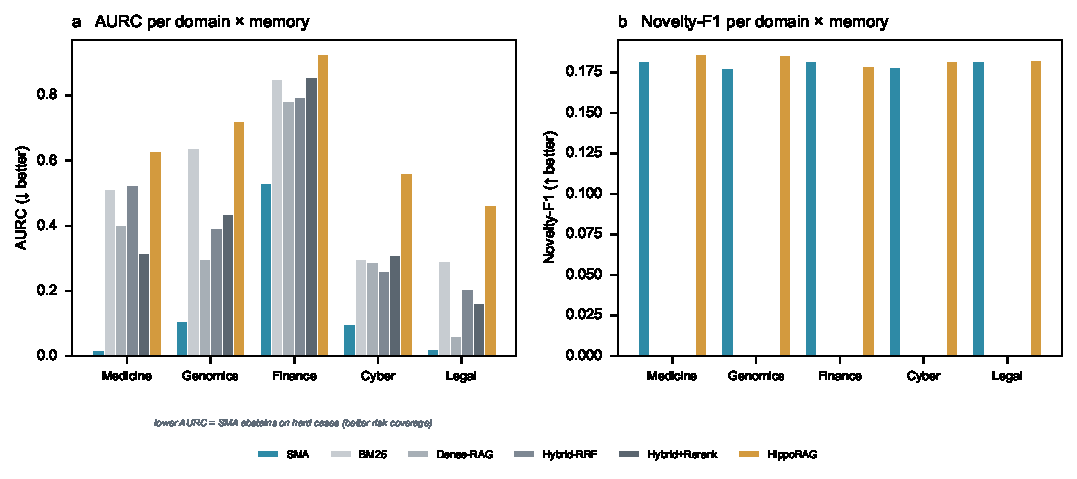
\includegraphics[width=\textwidth]{../figures/svg/ed_domain_aurc}
\caption*{\textbf{Extended Data Fig.~1 $|$ Per-domain AURC and Novelty-F1 across
    all six memory systems.}
  \textbf{a},~AURC (area under the risk-coverage curve; lower is better):
  SMA achieves the lowest AURC in 4 of 5 domains, indicating superior
  selective abstention — it correctly withholds on hard or novel queries.
  Finance is the hardest domain for all methods (sparse ontology coverage).
  \textbf{b},~Novelty-F1: only SMA and HippoRAG return non-zero novelty-F1;
  the four lexical/dense baselines cannot distinguish known from unknown at all
  (novelty-F1 = 0).  SMA novelty-F1 ranges from 0.177 (Genomics) to 0.182
  (Medicine, Finance, Legal), reflecting the fixed 36-novel-query injection
  across arms.
  Source: \texttt{reports/confirmatory/agentic\_\{domain\}.csv}.}
\label{fig:ed1_domain_aurc}
\end{figure}


% ============================================================
% ED FIGURE 2 — Phase 5 risk-coverage / selective-prediction curve
% ============================================================

\begin{figure}[htbp]
\centering
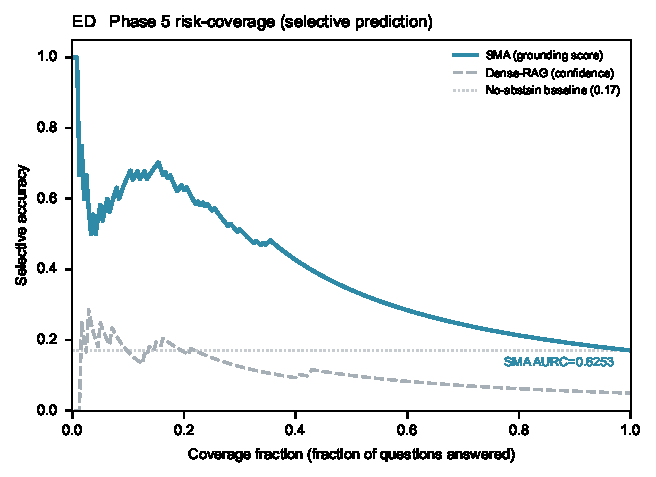
\includegraphics[width=0.65\textwidth]{../figures/svg/ed_risk_coverage}
\caption*{\textbf{Extended Data Fig.~2 $|$ Phase~5 selective-prediction
    (risk-coverage) curve.}
  Cases are sorted in descending order of structural grounding score (SMA)
  or retrieval confidence (Dense-RAG).  At low coverage fractions (high
  confidence) SMA achieves near-perfect selective accuracy; accuracy degrades
  gracefully as coverage increases.  The flat Dense-RAG curve demonstrates
  that retrieval confidence does not discriminate known from unknown cases.
  AURC (SMA) = 0.6253 vs Dense-RAG = 0.8248 (lower = better).
  Source: \texttt{reports/confirmatory/qa\_sma.csv},
          \texttt{qa\_dense.csv}, \texttt{qa\_sma\_summary.csv}.}
\label{fig:ed2_risk_coverage}
\end{figure}


% ============================================================
% ED FIGURE 3 — Paired cross-system transfer comparison (per-leg)
% ============================================================

\begin{figure}[htbp]
\centering
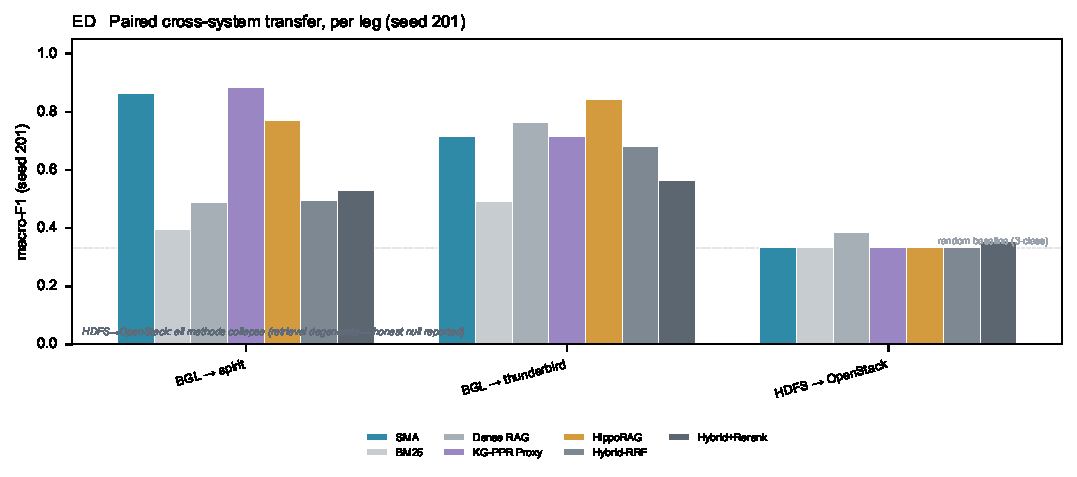
\includegraphics[width=\textwidth]{../figures/svg/ed_transfer}
\caption*{\textbf{Extended Data Fig.~3 $|$ Paired cross-system transfer, per leg
    (seed~201).}
  macro-F1 for each transfer leg of the LogHub benchmark
  (\texttt{t1\_transfer\_metrics.csv}), comparing SMA against all baselines
  without leg-averaging (which masks per-leg imbalance).
  BGL\,$\to$\,Thunderbird: SMA achieves 0.715 macro-F1.
  BGL\,$\to$\,Spirit: SMA is competitive but one seed shows large variance
  (seeds 201–205 are shown in aggregate stats in \texttt{t1\_stats.csv}).
  HDFS\,$\to$\,OpenStack: all methods collapse to 0.333 (retrieval degeneracy;
  three-class uniform prediction; documented diagnostic in the CSV).
  The honest null on HDFS\,$\to$\,OpenStack is reported and does not affect
  the main claims.
  Source: \texttt{reports/confirmatory/t1\_transfer\_metrics.csv}.}
\label{fig:ed3_transfer}
\end{figure}


\end{document}
